% Standalone TikZ diagram: simple unity-feedback closed-loop system.
% Build:  pdflatex closed_loop.tex
%
% Naming convention used throughout the book:
%   R(s)  reference     C(s)  controller
%   E(s)  error         G(s)  plant
%   U(s)  control       Y(s)  output

\documentclass[border=4pt]{standalone}
\usepackage{tikz}
\usetikzlibrary{positioning, calc, arrows.meta}

\begin{document}
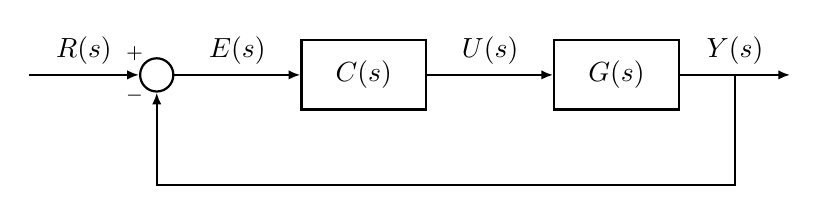
\begin{tikzpicture}[
  >={Latex[length=1.5mm, width=1.2mm]}, thick,
  block/.style = {draw, rectangle, minimum height=2.5em, minimum width=4.5em},
  sum/.style   = {draw, circle, inner sep=0pt, minimum size=1.2em},
]
  \node[coordinate]                    (rin)   {};
  \node[sum,   right=1.4cm of rin]     (sum)   {};
  \node[block, right=1.6cm of sum]     (C)     {$C(s)$};
  \node[block, right=1.6cm of C]       (G)     {$G(s)$};
  \node[coordinate, right=1.4cm of G]  (yout)  {};

  \node[font=\scriptsize, inner sep=0pt, anchor=south east] at (sum.north west) {$+$};
  \node[font=\scriptsize, inner sep=0pt, anchor=north east] at (sum.south west) {$-$};

  \draw[->] (rin) -- node[above]{$R(s)$} (sum);
  \draw[->] (sum) -- node[above]{$E(s)$} (C);
  \draw[->] (C)   -- node[above]{$U(s)$} (G);
  \draw[->] (G)   -- node[above]{$Y(s)$} (yout);

  \coordinate (fbk) at ($(G.east)!0.5!(yout)$);
  \draw[->] (fbk) -- ++(0,-1.4) -| (sum.south);
\end{tikzpicture}
\end{document}
